\chapter{Introduction}
\label{ch:introduction} 
A \acf{SPL} is outlined as a collection of similar software intensive systems
that share a set of common features satisfying the wants of specific customers, market segments 
or mission. Those similar software systems are developed from a set of core assets, comprised of 
documents, specifications, components, and other software artifacts that may be reusable throughout 
the development of each system within the product line
\citep{rafael2013systems}.

Requirements are typical assets in \ac{SPL}. They are specified in reusable models,
in which commonalities and variabilities are documented explicitly. Thus, these 
requirements can be instantiated and adapted to derive the requirements for an 
individual product \citep{cheng2007research}. New products in the SPL will be
much simpler to specify, because the requirements are reused and tailored
\citep{clements2002software}.

\acf{RE} in \ac{SPL} has an additional cost. Many \ac{SPL} requirements are
complex, interlinked, and divided into common, variable and product-specific requirements 
\citep{birk2003report,de2014defining}.  The requirements engineering process
must be tool-supported to handle complexity and the huge volume of elicited requirements
\citep{birk2003report}.

The focus of this dissertation is to provide a support tool for performing the specification of the 
\ac{SPL} requirements in a systematic way through the use of guidelines,  showing step by step how the 
specification should be done.

This chapter contextualizes the focus of this dissertation and starts by
presenting its motivation in \secref{sc:motivation} and a clear definition of the problem in 
\secref{sc:problem}. A brief overview of the proposed solution is presented in
\secref{sc:related}, while \secref{sc:outofscope} describes some aspects that
are not directly addressed by this work.
\secref{sc:contributions} presents the main contributions,  
\secref{sc:design} presents the research design  and, finally,
\secref{sc:structure} outlines the structure of this dissertation.

\section{Motivation}
\label{sc:motivation}


\section{Problem Statement}
\label{sc:problem}


\section{Related Work}
\label{sc:related}
In order to accomplish the goal of this dissertation, we propose the \acf{SPLICE}.
This tool supports the \acf{SPL} process activities in order to assist engineers in the traceability, variability management and maintenance activity.
The remainder of this section presents the context where it was developed and the outline of the proposed solution.

\subsection{Context}
This dissertation describes a tool that is part of the \ac{RiSE} \citep{Almeida2004}, formerly
called RiSE Project, whose goal is to develop a robust framework for software
reuse in order to enable the adoption of a reuse program. RiSE Labs it is
influenced by a series of areas, such as software measurement, architecture,
quality, environments and tools, and so on, in order to achieve its goal. The
influence areas can be seen in \figref{fg:rise-spiral}.

%\usepackage{graphics} is needed for \includegraphics
\begin{figure}[htp]
\begin{center}
  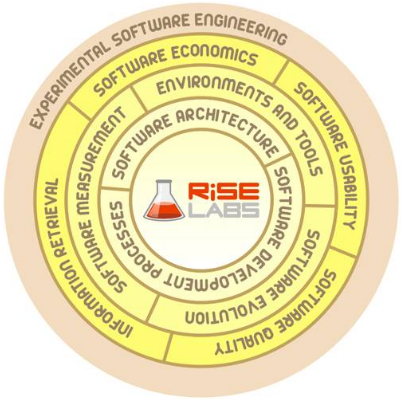
\includegraphics[width=9cm]{chapters/introduction/rise-spiral.png}
  \caption[RiSE Labs Influences]{RiSE Labs Influences}
  \label{fg:rise-spiral}
\end{center}
\end{figure}

Based on these areas, the RiSE Labs is divided in several projects, as shown in
Figure \ref{fg:rise-projects}. As it can be seen, this framework embraces
several different projects related to software reuse and software engineering.
They are:

\begin{itemize}
  \item \textbf{RiSE Framework:} Involves reuse processes
  \citep{Almeida2004,Nascimento2008}, component certification
  \citep{Alvaro2006} and reuse adoption process \citep{Garcia2008a}.
  
   \item \textbf{RiSE Tools:} Research focused on software reuse tools, such
   as the Admire Environment \citep{Mascena2006}, the Basic Asset Retrieval
   Tool (B.A.R.T) \citep{Santos2006}, which was enhanced with folksonomy
   mechanisms \citep{Vanderlei2007}, semantic layer \citep{Durao2008},
   facets \citep{Mendes2008} and data mining \citep{Martins2008}, and the
   Legacy InFormation retrieval Tool (LIFT) \citep{Brito2007}, the
   Reuse Repository System (CORE) \citep{CoreICSR}, and the Tool for Domain
   Analysis (ToolDAy) \citep{lisboa:msc:2008}. This dissertation is part of the RiSE tools;
   
   \item \textbf{RiPLE:}  Stands for RiSE Product Line Engineering Process and aims at developing   a methodology for Software Product Lines, composed of scoping \citep{Moraes2010},   requirements engineering \citep{neiva:msc:2009}, design \citep{filho:msc:2010,Cavalcanti:2011:ERP:2000259.2000286} , implementation, test \citep{neto:msc:2010,machado:msc:2010}, and evolution  management \citep{oliveira2009}.
   
   
   
   \item \textbf{SOPLE:} Development of a methodology for Service-Oriented Product Lines, based on the fundamentals of the RiPLE \citep{ribeiro2010}. 
   
   
   \item \textbf{MATRIX:} Investigates the area of measurement in reuse and
   its impact on quality and productivity;
   
   \item \textbf{BTT:} Research focused on tools for detection of duplicate
   bug reports, such as in \citet{CavalcantiFISL2008,CavalcantiInTech2012}.
   
   \item \textbf{Exploratory Research:} Investigates new research directions
   in software engineering and its impact on reuse;

   \item \textbf{CX-Ray:} Focused on understanding the \ac{C.E.S.A.R.}, and its
   processes and practices in software development.
\end{itemize}

This dissertation is part of the \ac{RiSE} Tools project. It was conducted in collaboration with researchers in software reuse , to solve the problem of traceability during the life-cycle of a\acf{SPL} development.


\begin{figure}[htp]
\begin{center}
  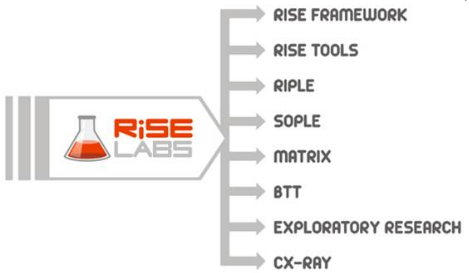
\includegraphics[width=10cm]{chapters/introduction/rise-projects.png}
  \caption[RiSE Labs Projects]{RiSE Labs Projects}
  \label{fg:rise-projects}
\end{center}
\end{figure}

\subsection{Outline of the Proposal}
This work defines the requirements, design and implementation of a software product lines lifecycle management tool, providing traceability and variability management and supporting most of the SPL process activities such as scoping, requirements, architecture, testing, version control, evolution, management and agile practices. In order to address it, we propose a metamodel that covers the SPL lifecycle, and develop a solution that consists in a Web based, extensible SPL lifecycle management tool, implementing this metamodel.  

The tool must enable the engineers involved in the process, to automatize the assets creation and maintenance, while providing traceability and variability management between them, providing detailed reports and enable the engineers to easily navigate between the assets using the traceability links. It must also provide a basic infrastructure for development, and a centralized point for user management among different tools.


\section{Out of Scope}
\label{sc:outofscope}
The following topics are not considered in the scope of this dissertation: 
\begin{itemize}
\item \textbf{SPL Domain Requirements Evolution}

Although an approach has already been proposed for the SPL domain requirements
evolution phase (FeDRE2), we still do not support this approach, but it is certainly a 
direction we intend to follow in the future.
\item \textbf{SPL Application Requirements Engineering}

In this work we do not consider the SPL Application Engineering process, then our contributions do 
not cover  the \ac{SPL} Application Requirements Engineering.
\item \textbf{Non-SPL Tools}

This work is concerned with Software Product Lines development and tools and
environments that support the \ac{SPL} approach. Non-SPL tools are out of scope.
\end{itemize}

\section{Statement of the Contributions}
\label{sc:contributions}
As a result of the work presented in this dissertation, the following contribution can be highlighted:
\begin{itemize}
\item \textbf{Tool support for a SPL domain requirements specification approach
(FeDRE)} 
We extended the \ac{SPLICE} tool, a \ac{SPL} lifecycle management tool
and automated \acf{FeDRE}, thus improving the automation of Software Product Lines (\ac{SPL}) requirements engineering phase.
\end{itemize}

\section{Research Design}
\label{sc:design}

The first step of our work was to investigate the software product line area. This informal 
study also included to understand the requirements engineering phase for single systems and 
software product lines. As a result, we could write out the second chapter with some foundations 
on these subjects.
 
During the informal study we identified the need for tools that appropriately support the domain 
requirements engineering phase of software product lines. After choosing a requirements specification 
approach (\ac{FeDRE}), we extended an existing SPL lifecycle management tool (\ac{SPLICE}) providing tool support 
for this approach.

In order to evaluate the proposed tool, we conducted a survey to identify limitations and needed 
improvements for the tool.  

\section{Dissertation Structure}
\label{sc:structure}
The remainder of this dissertation is organized as follows:

\begin{itemize}
\item \textbf{ Chapter \ref{ch:background} } reviews the essential topics
related to this work: Software Product Lines \ac{SPL}; requirements
engineering; \ac{SPL} requirements engineering; and \ac{SPLE} tool support.

\item \textbf{ Chapter \ref{ch:tool} } describes the \ac{SPLICE} tool, its
architeture and the set of frameworks and technologies used during its development. Also,  presents the new functional and non-functional 
requirements proposed for \ac{FeDRE} implementation based upon \ac{SPLICE}.

\item \textbf{ Chapter \ref{ch:survey} } describes an evaluation of \ac{FeDRE}
implementation.

\item \textbf{ Chapter \ref{ch:conclusion} } provides the concluding remarks. It
discusses our contributions, limitations, threats to validity, and outlines directions for future work.




\end{itemize}

